\documentclass[a4paper,11pt]{article}
\usepackage[utf8]{inputenc}
\usepackage[T1]{fontenc}
\usepackage[brazil]{babel}
\usepackage{graphicx}
\usepackage{amsmath}
\usepackage[bottom=2.0cm,top=2.0cm,left=2.0cm,right=2.0cm]{geometry}
\usepackage{indentfirst}
\usepackage{hyperref}
\usepackage{float}
\usepackage{subcaption}
\usepackage{booktabs}
\usepackage{tabularx}
\usepackage{siunitx}
\usepackage{xcolor}
\usepackage{listings}
\usepackage{tikz}
\usepackage{pgfplots}
\pgfplotsset{compat=1.18}
\usetikzlibrary{arrows.meta,positioning,calc}
\hypersetup{colorlinks,citecolor=black,filecolor=black,linkcolor=black,urlcolor=black}
\graphicspath{{./figuras/}}
\setlength{\parskip}{0.45em}
\sisetup{output-decimal-marker={,}, group-minimum-digits=4}

\lstset{basicstyle=\ttfamily\footnotesize, frame=single, columns=fullflexible,
        keepspaces=true, showstringspaces=false, language=C}

% Common TikZ styles (same as the ideation report)
\tikzset{
  blk/.style={draw, fill=black!85, text=white, rounded corners=1pt, minimum height=9mm,
              minimum width=22mm, align=center, font=\footnotesize\bfseries},
  sumc/.style={draw, circle, minimum size=6mm, inner sep=0pt},
  sig/.style={-{Latex[length=2mm]}, thick},
  hw/.style={draw, thick, rounded corners=2pt, align=center, font=\footnotesize, fill=gray!10},
  wire/.style={thick},
}

% Photo of the prototype: put figuras/foto_prototipo.jpg (or .png) and recompile.
\newcommand{\fotoprototipo}[1]{%
  \IfFileExists{figuras/foto_prototipo.jpg}{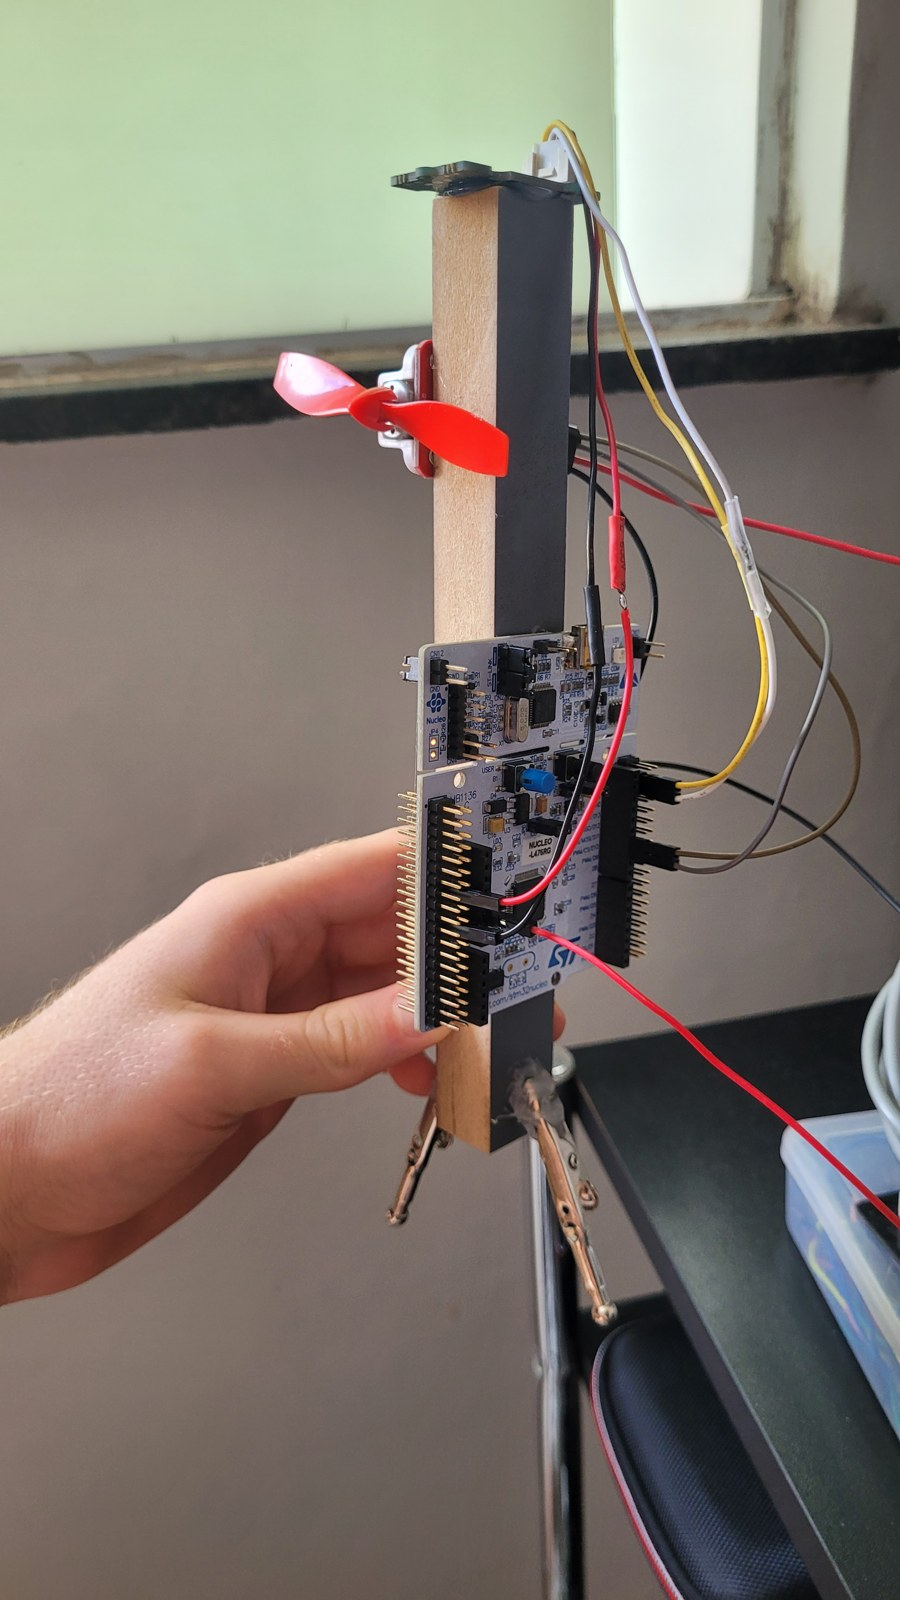
\includegraphics[height=#1]{foto_prototipo.jpg}}{%
  \IfFileExists{figuras/foto_prototipo.png}{\includegraphics[height=#1]{foto_prototipo.png}}{%
  \fbox{\parbox[c][#1][c]{0.85\linewidth}{\centering\small\itshape
        Espaço para a foto do protótipo\\(salvar como \texttt{figuras/foto\_prototipo.jpg})}}}}}

\begin{document}

%%%%%%%%%%%%%%%%%%%%%%%%%%%%%%%%%%%%%%%%%%%%%%%%%%%%%%%%%%%%%%%%%%%%%%%%%%%%
\noindent
\begin{minipage}[c]{0.16\textwidth}
  
\includegraphics[width=\linewidth]{brasao_ufba.png}
\end{minipage}\hfill
\begin{minipage}[c]{0.82\textwidth}
  \raggedleft
  {\small Universidade Federal da Bahia -- Escola Politécnica}\\
  {\small ENGC54 -- Laboratório Integrado VI (Controle) -- Prof.\textsuperscript{a} Cristiane Paim}\\[3pt]
  {\small João Pedro Penelu \quad $\cdot$ \quad Davi Buente}\\
  {\small 11 de novembro de 2026}
\end{minipage}

\vspace{10pt}
\begin{center}
  {\LARGE\textbf{AeroPêndulo}}\\[2pt]
  {\large Controle do ângulo de uma haste por propulsão a hélice}\\[2pt]
  {\normalsize\itshape Relatório parcial (TP2): protótipo, modelagem e \textit{anti-windup} atualizados}
\end{center}
\vspace{-4pt}

%%%%%%%%%%%%%%%%%%%%%%%%%%%%%%%%%%%%%%%%%%%%%%%%%%%%%%%%%%%%%%%%%%%%%%%%%%%%
\section{Introdução}

Este relatório parcial atualiza a proposta inicial do AeroPêndulo (TP1), uma haste apoiada no piso
por dois pontos, que só tomba em um eixo e cujo ângulo é mantido por uma hélice, e o estudo de
\textit{anti-windup} por integração limitada feito pela equipe (AS). Desde então, foi construído e
ensaiado um primeiro protótipo (v1). Os ensaios confirmaram a arquitetura de controle e o
\textit{firmware}, mas revelaram três limitações físicas do conjunto: empuxo muito menor que o
previsto, aquecimento excessivo do \textit{driver} do motor e estrutura pesada demais.

O relatório apresenta: o que mudou em relação à ideação (Seção~\ref{sec:evolucao}); o protótipo v1 e o
\textit{firmware} (Seções~\ref{sec:prototipo} e~\ref{sec:firmware}); os ensaios de bancada e a análise
em malha aberta (Seção~\ref{sec:ensaios}); a modelagem matemática com os parâmetros medidos
(Seção~\ref{sec:modelo}); a revisão do \textit{anti-windup} para um atuador que só empurra em um
sentido, com simulação e modelo em Simulink (Seções~\ref{sec:aw} e~\ref{sec:simulink}); os objetivos
específicos do controlador (Seção~\ref{sec:objetivos}); e os próximos passos até a entrega final
(Seção~\ref{sec:proximos}).

%%%%%%%%%%%%%%%%%%%%%%%%%%%%%%%%%%%%%%%%%%%%%%%%%%%%%%%%%%%%%%%%%%%%%%%%%%%%
\section{Evolução da proposta}
\label{sec:evolucao}

A Tabela~\ref{tab:evolucao} compara a ideação, o protótipo construído e o protótipo planejado
para a etapa final. A mudança mais importante é o \textbf{atuador unidirecional}: na ideação, o
motor giraria nos dois sentidos para corrigir quedas para os dois lados. Na prática, o sentido
reverso da hélice fornece menos da metade do empuxo e as inversões rápidas sobreaqueceram o
\textit{driver}. A haste passa então a operar \textbf{levemente inclinada} ($\theta_{ref}<90^\circ$):
a gravidade fornece a força de retorno e a hélice só empurra no sentido mais eficiente.

\begin{table}[!htb]
\centering\small
\caption{Evolução da proposta: ideação (TP1), protótipo construído (v1) e protótipo planejado (v2).}
\label{tab:evolucao}
\begin{tabularx}{\textwidth}{@{}l>{\raggedright}X>{\raggedright}X>{\raggedright\arraybackslash}X@{}}
\toprule
\textbf{Item} & \textbf{Ideação (TP1)} & \textbf{Protótipo v1 (construído)} & \textbf{Protótipo v2 (planejado)} \\
\midrule
Estrutura & PLA impresso em 3D & haste de MDF com a Nucleo e os fios embarcados & haste leve de PLA, só com IMU e ventilador \\
Sensor & acelerômetro no topo & IMU MPU-9250 (acelerômetro + giroscópio), I\textsuperscript{2}C & mesma IMU, \textbf{perto do pivô} \\
Atuador & motor DC + hélice, bidirecional & ventilador QYF-749 (5 V, hélice 75 mm) & motor com mais empuxo (a avaliar) \\
\textit{Driver} & ponte H L9110S & ponte H L9110H & MOSFET de nível lógico (sem ponte H) \\
Sentido do empuxo & dois sentidos & só para frente ($u\ge 0$) & só para frente \\
Alimentação do motor & fonte 3--6 V & bateria 9 V (descartada) $\rightarrow$ fonte 5 V / 2 A & fonte 5 V / 2 A \\
Referência & $90^\circ$ (vertical) & $85^\circ$, ou o ângulo atual ao apertar o botão B1 & $83^\circ$ a $88^\circ$ \\
Controlador & PID digital & PID 200 Hz, D pelo giroscópio, integração limitada & idem, ganhos ajustados \\
\bottomrule
\end{tabularx}
\end{table}

%%%%%%%%%%%%%%%%%%%%%%%%%%%%%%%%%%%%%%%%%%%%%%%%%%%%%%%%%%%%%%%%%%%%%%%%%%%%
\section{Protótipo construído (v1)}
\label{sec:prototipo}

O protótipo v1 (Figura~\ref{fig:prototipo}a) usa uma haste de MDF apoiada no piso por duas pontas
arredondadas. No topo ficam a IMU e o ventilador; a placa NUCLEO-L476RG e o módulo do motor foram
presos à própria haste. A Figura~\ref{fig:prototipo}b mostra o projeto em PLA do estudo de
\textit{anti-windup}, que serve de base para o protótipo v2.

\begin{figure}[H]
\centering
\begin{subfigure}[b]{0.48\textwidth}
  \centering
  \fotoprototipo{6.0cm}
  \caption{Protótipo v1 construído.}
\end{subfigure}\hfill
\begin{subfigure}[b]{0.48\textwidth}
  \centering
  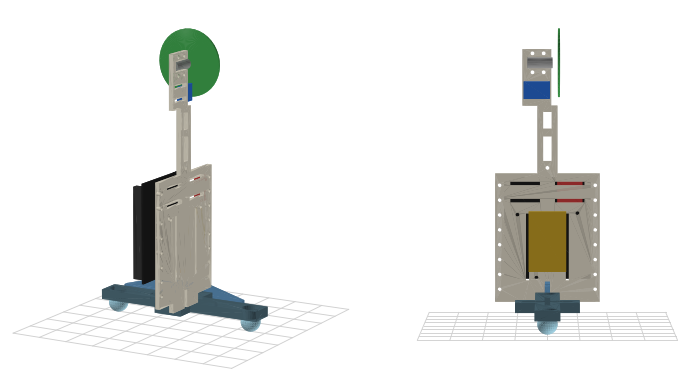
\includegraphics[width=\linewidth,height=6.0cm,keepaspectratio]{cad_prototipo_pla.png}
  \caption{Projeto em PLA (base do v2).}
\end{subfigure}
\caption{(a) Protótipo v1; (b) modelo CAD da haste em PLA usado no estudo de \textit{anti-windup}.}
\label{fig:prototipo}
\end{figure}

A Figura~\ref{fig:ligacoes} e a Tabela~\ref{tab:pinos} mostram as ligações elétricas. A IMU é
alimentada em 3,3~V pela Nucleo, e o motor por uma fonte externa de 5~V com terra comum. A Nucleo é
alimentada pelo USB, que também leva a comunicação serial com o PC.

\begin{figure}[H]
\centering
\begin{tikzpicture}[every node/.style={font=\scriptsize}]
  \node[hw, fill=black!80, text=white, minimum width=20mm, minimum height=44mm] (nuc) at (0,0)
       {\textbf{NUCLEO}\\\textbf{L476RG}\\[2mm]botão B1\\(PC13)};
  \node[hw, anchor=west, minimum height=14mm] (imu) at (4.4,1.4)
       {\textbf{IMU MPU-9250}\\(I\textsuperscript{2}C 0x68)};
  \node[hw, anchor=west, minimum height=14mm] (drv) at (4.4,-1.3)
       {\textbf{Módulo L9110H}\\(ponte H)};
  \node[draw, thick, circle, minimum size=8mm, right=12mm of drv] (mot) {\textbf{M}};
  \draw[very thick] ($(mot)+(0,0.75)$) -- ($(mot)+(0,-0.75)$);
  \node[below=6mm of mot] {ventilador QYF-749};
  \node[hw, anchor=west, minimum height=8mm] (src) at (4.4,-3.4) {Fonte 5 V / 2 A};
  \node[hw, minimum width=11mm] (pc) at (-3.8,0) {PC};

  \foreach \y/\lbl in {1.85/3V3, 1.4/{D14 -- SDA}, 0.95/{D15 -- SCL}}
    \draw[wire, blue] (1.0,\y) -- node[above=-1.5pt]{\lbl} (4.4,\y);
  \foreach \y/\lbl in {-1.05/{D10 $\rightarrow$ INA (PWM)}, -1.55/{D11 $\rightarrow$ INB (PWM)}}
    \draw[wire, red] (1.0,\y) -- node[above=-1.5pt]{\lbl} (4.4,\y);
  \draw[wire] ($(drv.east)+(0,0.2)$) -- ($(mot.west)+(0,0.2)$);
  \draw[wire] ($(drv.east)+(0,-0.2)$) -- ($(mot.west)+(0,-0.2)$);
  \draw[wire, orange!80!black] (src.north -| drv.south) -- node[right]{VCC 5 V} (drv.south);
  \draw[wire, dashed] (nuc.south) |- node[pos=0.7, below]{GND comum} (src.west);
  \draw[wire, {Latex}-{Latex}] (pc.east) -- node[above]{USB} node[below]{UART 115200} (nuc.west);
\end{tikzpicture}
\caption{Ligações do protótipo v1. PWM de 20~kHz nas duas entradas da ponte H.}
\label{fig:ligacoes}
\end{figure}

\begin{table}[H]
\centering\small
\caption{Pinagem usada na NUCLEO-L476RG.}
\label{tab:pinos}
\begin{tabular}{@{}lll@{}}
\toprule
\textbf{Função} & \textbf{Pino (Arduino)} & \textbf{STM32} \\
\midrule
IMU SDA / SCL & D14 / D15 & PB9 / PB8 (I\textsuperscript{2}C1, 100 kHz) \\
Motor INA / INB & D10 / D11 & PB6 (TIM4\_CH1) / PA7 (TIM3\_CH2), 20 kHz \\
Botão de usuário & B1 & PC13 \\
LED de estado & LD2 & PA5 \\
Serial com o PC & USB (ST-LINK) & USART2, 115200 8N1 \\
\bottomrule
\end{tabular}
\end{table}

%%%%%%%%%%%%%%%%%%%%%%%%%%%%%%%%%%%%%%%%%%%%%%%%%%%%%%%%%%%%%%%%%%%%%%%%%%%%
\section{\textit{Firmware} e ferramentas}
\label{sec:firmware}

O \textit{firmware} (C, HAL da ST, sem RTOS) roda um laço fixo de 200~Hz ($T_s=5$~ms):
\begin{enumerate}
  \item lê a IMU (±4~g, ±500~°/s, filtro interno de 41~Hz);
  \item estima o ângulo com um filtro complementar,
    $\hat\theta[k]=\alpha\big(\hat\theta[k-1]+\omega[k]T_s\big)+(1-\alpha)\,\theta_{acc}[k]$, com
    $\theta_{acc}=\operatorname{atan2}(a_{up},a_{side})$ e constante de tempo de 0,5~s;
  \item calcula o PID com o termo derivativo pela taxa do giroscópio e o integrador limitado
    (Seção~\ref{sec:aw});
  \item aplica a compensação de zona morta e o teto de razão cíclica, e envia telemetria a 50~Hz.
\end{enumerate}

Por segurança, o motor desliga em três situações: no comando \texttt{stop}, em erro de leitura da
IMU e em queda ($|\theta-90^\circ|>30^\circ$). O botão B1 liga o controle tomando o ângulo atual como
referência. Se o controle já estiver ligado, o mesmo botão funciona como parada de emergência. A
referência, os ganhos, os limites do integrador e o teto de PWM podem ser alterados pela serial.

Para tornar os ensaios reprodutíveis, foi criado um \textit{script} de bancada em Python
(\texttt{teste\_bancada.py}). Cada etapa (placa, IMU, eixos, motor, sinal, botão e empuxo) é um
teste guiado, com critérios numéricos de aprovação e registro automático dos resultados. Um
aplicativo no PC mostra o ângulo, a referência e o sinal de controle em tempo real e exporta CSV.

%%%%%%%%%%%%%%%%%%%%%%%%%%%%%%%%%%%%%%%%%%%%%%%%%%%%%%%%%%%%%%%%%%%%%%%%%%%%
\section{Ensaios de bancada e análise em malha aberta}
\label{sec:ensaios}

\subsection{Sensor e acionamento}

A Tabela~\ref{tab:ensaios} resume os ensaios. A IMU e o caminho do PWM foram validados. A bateria de
9~V foi descartada porque a tensão caiu 34\,\% com o motor ligado, e foi substituída por uma
fonte de 5~V, cuja queda em carga máxima foi de só 3\,\%.

\begin{table}[H]
\centering\small
\caption{Resultados dos ensaios de bancada (protótipo v1).}
\label{tab:ensaios}
\begin{tabularx}{\textwidth}{@{}l>{\raggedright}Xl@{}}
\toprule
\textbf{Ensaio} & \textbf{Resultado} & \textbf{Situação} \\
\midrule
Ruído do giroscópio em repouso & 0,07--0,08~°/s (desvio-padrão) & OK ($<0{,}3$~°/s) \\
\textit{Bias} do giroscópio após calibração & $\le 0{,}02$~°/s & OK \\
Ruído do acelerômetro & 0,002--0,004~g & OK \\
Mapeamento dos eixos & up $+z$, side $-y$, giro $+x$; giroscópio coerente com o acelerômetro & OK \\
PWM aplicado $\times$ comandado (10--100\,\%) & iguais nos dois sentidos & OK \\
Bateria 9~V com o motor em 55\,\% & 9~V $\rightarrow$ 5,9~V (queda de 34\,\%) & descartada \\
Fonte 5~V com o motor em 100\,\% & 4,85~V (queda de 3\,\%) & OK \\
Início do giro da hélice (5~V) & $\approx 30\,\%$ de razão cíclica nos dois sentidos & zona morta \\
Empuxo máximo (90\,\%) & 9~gf (0,088~N) no sentido forte; 4~gf no outro & \textbf{baixo} \\
Temperatura do módulo L9110H & muito quente após poucos segundos & \textbf{inviável} \\
\bottomrule
\end{tabularx}
\end{table}

\subsection{Curva de empuxo}

O empuxo foi medido com uma balança de cozinha (resolução de 1~g), com o ventilador soprando para
cima, em degraus de 10\,\% de razão cíclica (Figura~\ref{fig:empuxo}). A hélice é fortemente
assimétrica: o sentido mais eficiente fornece mais que o dobro do empuxo do outro. Embora a
hélice comece a girar em cerca de 30\,\%, o empuxo só passa de 1~g acima de 50 a 60\,\%. A curva tem
forma aproximadamente quadrática, como esperado para uma hélice.

\begin{figure}[H]
\centering
\begin{tikzpicture}
\begin{axis}[width=0.62\textwidth, height=5.2cm, xlabel={Razão cíclica (\%)}, ylabel={Empuxo (gf)},
             xmin=25, xmax=95, ymin=-0.5, ymax=10, grid=major, legend pos=north west,
             legend style={font=\footnotesize}, tick label style={font=\footnotesize}]
  \addplot[blue!70!black, thick, mark=*] coordinates {(40,0) (50,1) (60,2) (70,3) (80,7) (90,9)};
  \addlegendentry{sentido forte (usado no controle)}
  \addplot[red!70!black, thick, mark=square*] coordinates {(30,0) (40,0) (50,1) (60,1) (70,1) (80,3) (90,4)};
  \addlegendentry{sentido oposto}
\end{axis}
\end{tikzpicture}
\caption{Curva de empuxo do ventilador QYF-749 a 5~V, acionado pelo L9110H (1~gf $=$ 9,81~mN).}
\label{fig:empuxo}
\end{figure}

O empuxo baixo e o aquecimento têm uma causa comum provável: o L9110H é uma ponte H de
transistores bipolares, com queda de tensão da ordem de 1~V e chaveamento lento para o PWM de
20~kHz. Assim, o motor recebe bem menos que 5~V e o \textit{driver} dissipa a diferença.

\subsection{Malha aberta e primeiros ensaios em malha fechada}

Sem controle, a haste cai em menos de um segundo para qualquer lado, como prevê o modelo
(polo instável, Seção~\ref{sec:modelo}). Nos primeiros ensaios em malha fechada, o ventilador
empurrou a haste \textbf{a favor} da queda. Era realimentação positiva, causada pelo sinal do motor
em relação ao ângulo, e foi corrigida no \textit{firmware} (\texttt{MOTOR\_SIGN\_DEFAULT}). Em
seguida, as inversões de sentido do PID aqueceram muito o L9110H. Por isso o atuador passou a operar
só para frente ($u\in[0,u_{max}]$), com teto de 90\,\% de razão cíclica.

Com a haste de MDF, a Nucleo, os fios e o cabo USB embarcados, o empuxo disponível não foi
suficiente para sustentar a haste. A análise da Seção~\ref{sec:modelo} mostra que essa conclusão é
quantitativa: o torque máximo da hélice é pequeno diante do torque da gravidade de uma haste pesada.
Por isso o equilíbrio em malha fechada ainda \textbf{não foi obtido} no protótipo v1, o que motivou
o redesenho descrito na Seção~\ref{sec:proximos}.

%%%%%%%%%%%%%%%%%%%%%%%%%%%%%%%%%%%%%%%%%%%%%%%%%%%%%%%%%%%%%%%%%%%%%%%%%%%%
\section{Modelagem matemática}
\label{sec:modelo}

Seja $\phi=\theta-90^\circ$ o desvio em relação à vertical. A segunda lei de Newton para a rotação
em torno do eixo dos apoios e uma dinâmica de primeira ordem para o conjunto motor--hélice dão
\begin{align}
  J\,\ddot\phi &= m g h \sin\phi - b\,\dot\phi + L\,F + \tau_d, \label{eq:planta}\\
  \tau_m\,\dot F &= \operatorname{sat}(u) - F,\qquad 0 \le \operatorname{sat}(u) \le F_{max}, \label{eq:atuador}
\end{align}
em que $J$ é o momento de inércia em torno do pivô, $m$ a massa total, $h$ a altura do centro de
massa, $L$ a altura do eixo da hélice, $b$ o atrito viscoso, $F$ o empuxo e $\tau_d$ um torque de
perturbação. Linearizando em torno de $\phi=0$ e desprezando $\tau_m$,
\begin{equation}
  G(s)=\frac{\Phi(s)}{F(s)}=\frac{L/J}{s^2+(b/J)\,s-mgh/J}.
  \label{eq:G}
\end{equation}
Com os parâmetros da Tabela~\ref{tab:param}, os polos ficam em $-9{,}68$ e $+9{,}22$~rad/s. O polo
no semiplano direito confirma que a planta é instável em malha aberta, com constante de tempo de
queda de cerca de 0,11~s.

\begin{table}[H]
\centering\small
\caption{Parâmetros do modelo. A haste é o projeto em PLA (base do v2); o atuador foi medido no v1.}
\label{tab:param}
\begin{tabular}{@{}llll@{}}
\toprule
\textbf{Símbolo} & \textbf{Valor} & \textbf{Descrição} & \textbf{Origem} \\
\midrule
$m$ & 0,145 kg & massa total & CAD \\
$h$ & 0,069 m & altura do centro de massa & CAD \\
$L$ & 0,212 m & altura do empuxo & CAD \\
$J$ & $1{,}10\times10^{-3}$ kg$\cdot$m$^2$ & inércia em torno do pivô & CAD \\
$b$ & $5\times10^{-4}$ N$\cdot$m$\cdot$s/rad & atrito viscoso & estimado \\
$\tau_m$ & 0,03 s & constante de tempo do atuador & estimado \\
$F_{max}$ & 0,088 N (9 gf) & empuxo máximo (90\,\% PWM) & \textbf{medido} \\
$F_{min}$ & 0 & atuador só para frente & decisão de projeto \\
$\phi_{bat}$ & $\pm 24^\circ$ & haste encostada no piso & CAD \\
\bottomrule
\end{tabular}
\end{table}

\textbf{Ponto de operação e viabilidade.} Para manter a haste parada em $\phi_r$, a hélice deve
fornecer o empuxo de sustentação
\begin{equation}
  F_h=-\frac{m g h \sin\phi_r}{L},
  \label{eq:Fh}
\end{equation}
que é positivo apenas para $\phi_r<0$ ($\theta_r<90^\circ$), já que o atuador só empurra em um
sentido. O maior desvio sustentável é
\begin{equation}
  |\phi|_{max}=\arcsin\!\left(\frac{F_{max}\,L}{m g h}\right)=\arcsin\!\left(\frac{0{,}088\times0{,}212}{0{,}145\times9{,}81\times0{,}069}\right)\approx 11^\circ .
  \label{eq:phimax}
\end{equation}
Mesmo com a haste leve de PLA, o ventilador atual só sustenta a haste entre $79^\circ$ e $90^\circ$,
e em $\theta_r=85^\circ$ já gasta $F_h=0{,}040$~N, 46\,\% do empuxo máximo. A expressão
\eqref{eq:phimax} também mostra o que fazer no protótipo v2: reduzir o produto $m\,h$ (haste leve,
com a Nucleo e o \textit{driver} fora dela e a IMU perto do pivô), aumentar $L$ (hélice no topo) e
aumentar $F_{max}$ (\textit{driver} sem queda de tensão e, se preciso, outro motor). A haste de MDF
do v1, com a placa embarcada, tem $m\,h$ várias vezes maior, o que explica por que ela não pôde
ser sustentada.

%%%%%%%%%%%%%%%%%%%%%%%%%%%%%%%%%%%%%%%%%%%%%%%%%%%%%%%%%%%%%%%%%%%%%%%%%%%%
\section{\textit{Anti-windup} revisado: atuador unidirecional}
\label{sec:aw}

\subsection{Por que o \textit{windup} ficou mais crítico}

No estudo de \textit{anti-windup}, o atuador era bidirecional e assimétrico
($-0{,}10$ a $0{,}25$~N). Agora ele é unidirecional ($0$ a $0{,}088$~N). Com $\theta_r<90^\circ$, a
hélice empurra a haste em direção à vertical e a gravidade a puxa de volta. Se a haste
\textbf{ultrapassar a vertical}, gravidade e empuxo passam a agir no mesmo sentido, e não há força
capaz de trazê-la de volta: ela tomba. Qualquer sobressinal que cruze $90^\circ$ é, portanto, fatal.
É exatamente o tipo de sobressinal que o \textit{windup} da ação integral produz depois de um período
de saturação.

A situação de saturação mais comum no uso do protótipo é a partida pelo botão B1: o usuário
segura a haste, aperta o botão e a solta. Enquanto a mão segura a haste abaixo da referência, o
erro é positivo, o atuador fica saturado em $F_{max}$ e o integrador acumula erro sem efeito sobre a
saída.

\subsection{Integração limitada e escolha dos limites}

A lei de controle implementada é
\begin{equation}
  I[k]=\min\!\Big(\max\big(I[k-1]+K_iT_s\,e[k],\;I_{min}\big),\;I_{max}\Big),\qquad
  u[k]=K_p\,e[k]+I[k]-K_d\,\omega[k],
  \label{eq:il}
\end{equation}
em que $\omega$ é a taxa medida pelo giroscópio. Em regime, $u_{ss}=I_{ss}=F_h$. Pela regra do
estudo de \textit{anti-windup}, os limites devem conter $F_h$ em toda a faixa de operação e ficar
dentro da faixa do atuador, com margem $\mu=25\,\%$. Para a faixa $83^\circ\le\theta_r\le 88^\circ$,
\eqref{eq:Fh} dá $0{,}016\le F_h\le 0{,}056$~N. Logo,
\begin{equation}
  I_{max}=\min\big(F_{max},\,(1+\mu)\max F_h\big)=\min(0{,}088;\;0{,}0705)=0{,}0705~\mathrm{N},
  \qquad I_{min}=F_{min}=0 .
\end{equation}
O limite inferior nulo é coerente com o atuador unidirecional: um termo integral negativo só
acumularia \textit{windup}, já que $u<0$ é cortado pela saturação. No \textit{firmware}, o trecho
correspondente é:

\begin{lstlisting}
float pid_step(pidc_t *c, float theta, float rate, float dt)
{
    float e = c->ref - theta;
    c->i = clamp(c->i + c->ki * dt * e, c->i_min, c->i_max);   /* limited integration */
    c->u = c->kp * e + c->i - c->kd * rate;                      /* D on the gyro rate  */
    c->u_sat = clamp(c->u, c->u_min, c->u_max);                  /* u_min = 0           */
    return c->u_sat;
}
\end{lstlisting}

\subsection{Simulação}

O modelo não linear \eqref{eq:planta}--\eqref{eq:atuador} foi simulado com o PID digital
\eqref{eq:il} ($T_s=5$~ms). Os ganhos foram mantidos os do estudo de \textit{anti-windup}, obtidos
por alocação de polos com $\omega_n=8$~rad/s, $\zeta=0{,}9$ e polo real em $-16$~rad/s:
$K_p=1{,}991$~N/rad, $K_i=5{,}313$~N/(rad$\cdot$s) e $K_d=0{,}155$~N$\cdot$s/rad. A haste parte em
equilíbrio em $\theta_r=85^\circ$. Entre 0,5 e 2,0~s, uma ``mão'', modelada como mola e amortecedor,
segura a haste em $82^\circ$ e depois a solta. Três casos são comparados:
\begin{itemize}
  \item[(a)] atuador ideal, sem saturação;
  \item[(b)] atuador medido ($0\le F\le 0{,}088$~N), sem \textit{anti-windup};
  \item[(c)] atuador medido, com integração limitada em $[0;\,0{,}0705]$~N.
\end{itemize}

\begin{figure}[H]
\centering
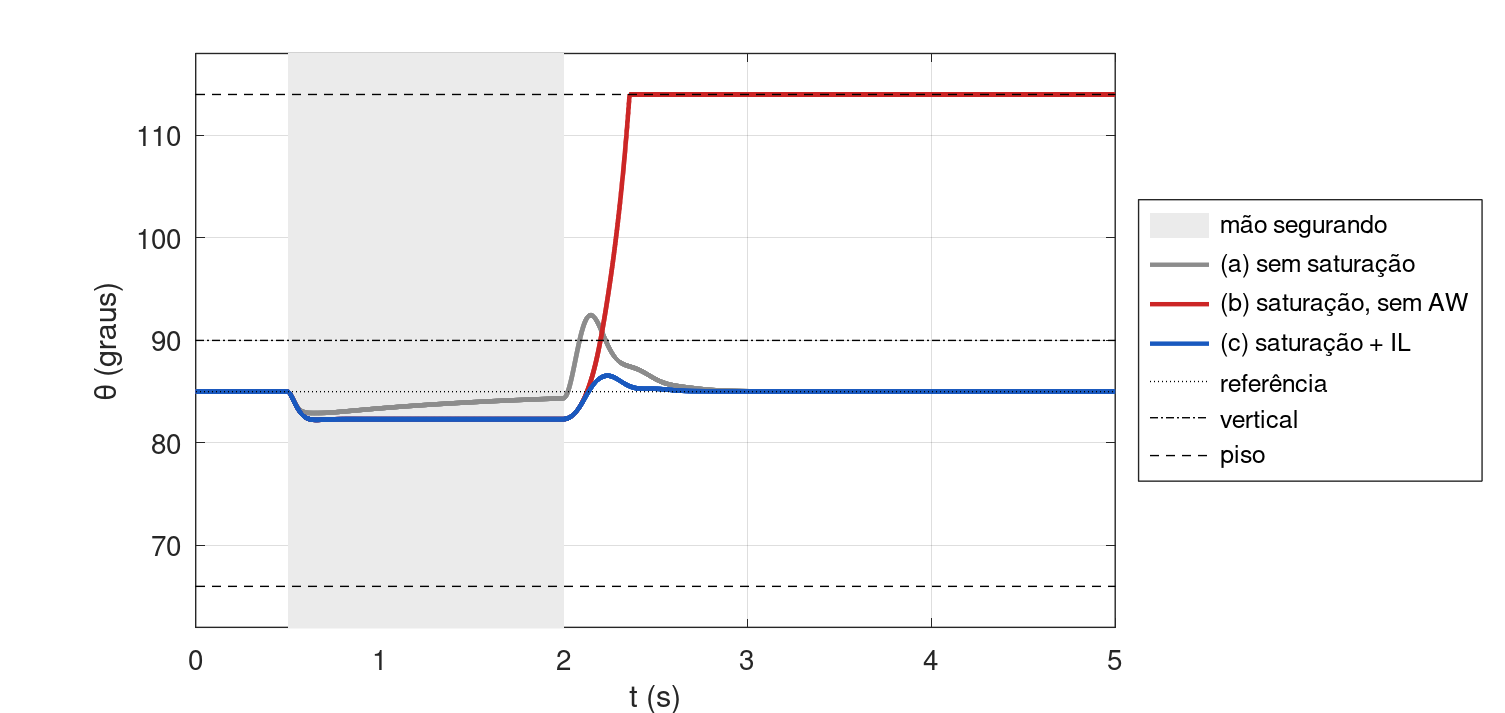
\includegraphics[width=0.86\textwidth]{fig_sim_angulo.png}
\caption{Ângulo da haste. Faixa cinza: a mão segura a haste em $82^\circ$. Tracejado: piso ($66^\circ$ e
$114^\circ$); traço-ponto: vertical.}
\label{fig:simang}
\end{figure}

\begin{figure}[H]
\centering
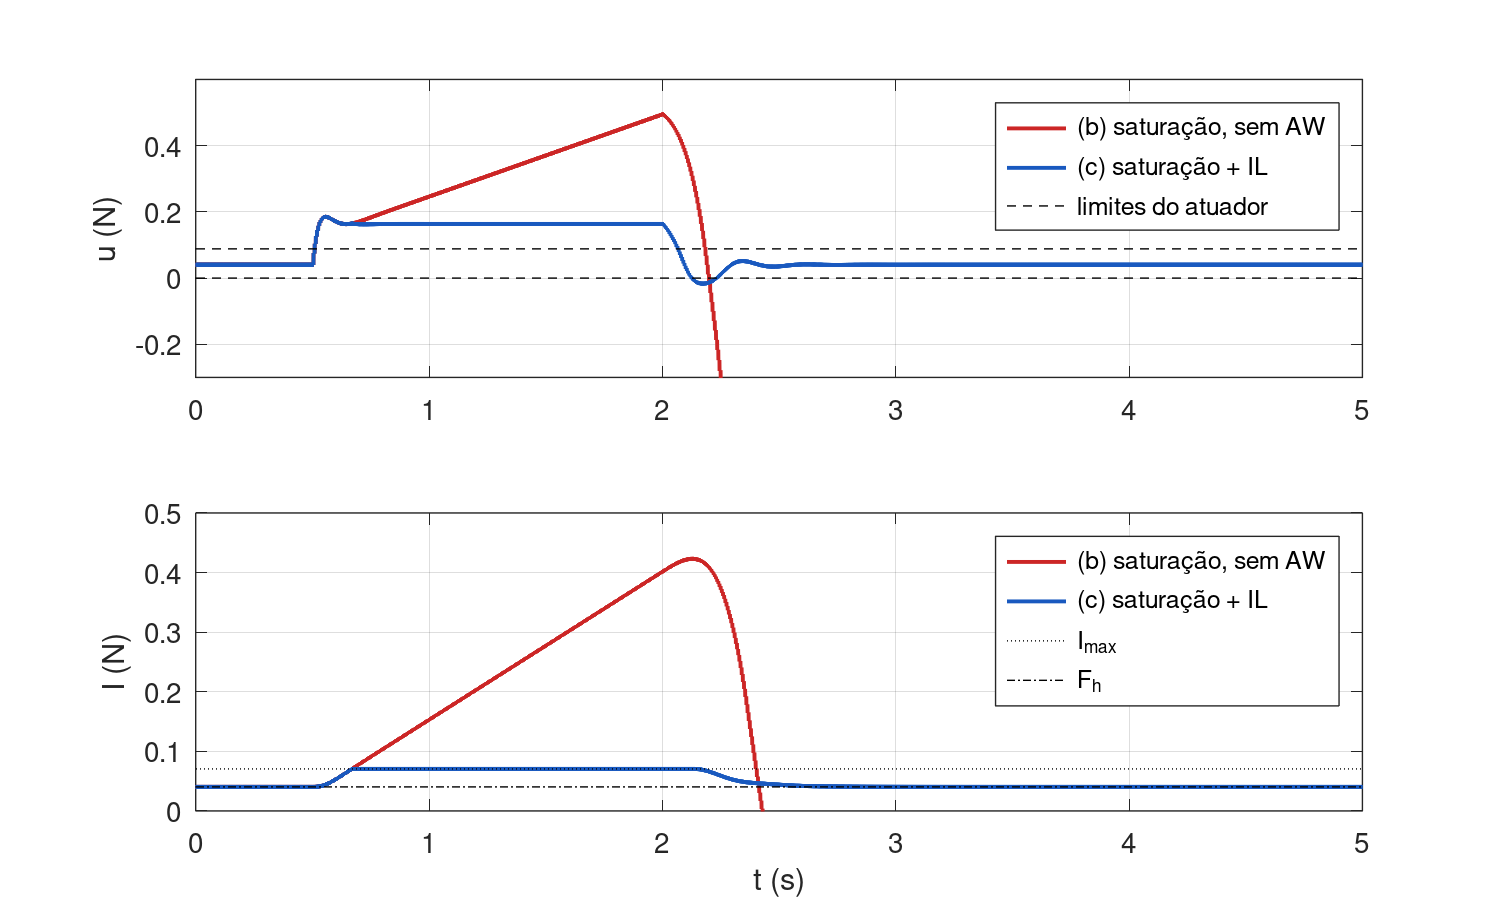
\includegraphics[width=0.80\textwidth]{fig_sim_controle.png}
\caption{Sinal de controle calculado $u$ (acima) e termo integral $I$ (abaixo) nos casos com saturação.}
\label{fig:simctrl}
\end{figure}

\begin{table}[H]
\centering\small
\caption{Desempenho após a mão soltar a haste ($t=2{,}0$~s). $t_r$: tempo até entrar
definitivamente na faixa de $\pm1^\circ$; IAE calculado a partir da soltura.}
\label{tab:sim}
\begin{tabular}{@{}lccccc@{}}
\toprule
\textbf{Caso} & $\theta_{max}$ ($^\circ$) & pico de $I$ (N) & $t_r$ (s) & IAE ($^\circ\cdot$s) & resultado \\
\midrule
(a) sem saturação & 92,5 & 0,223 & 0,53 & 2,0 & recupera \\
(b) saturação, sem AW & 114,0 & 0,423 & $\infty$ & 79,4 & \textbf{tomba} \\
(c) saturação + IL & 86,6 & 0,071 & 0,31 & 0,6 & recupera \\
\bottomrule
\end{tabular}
\end{table}

\textbf{Discussão.}
\begin{itemize}
  \item \textbf{Sem \textit{anti-windup} (b).} Enquanto a mão segura a haste, o integrador sobe de
    0,040 para 0,423~N, 4,8 vezes o empuxo máximo (Figura~\ref{fig:simctrl}). Ao soltar, esse excesso
    mantém o ventilador saturado, a haste cruza a vertical e tomba.
  \item \textbf{Com integração limitada (c).} O integrador para em 0,0705~N. A haste sobe só até
    $86{,}6^\circ$ e volta à faixa de $\pm1^\circ$ em 0,31~s.
  \item \textbf{Caso ideal (a).} Mesmo com atuador ilimitado, o integrador comum cresce e leva a haste
    a $92{,}5^\circ$. No atuador real, esse sobressinal derrubaria a haste.
  \item \textbf{Tempo segurando a haste.} Ele não altera o resultado da integração limitada: com a mão
    segurando por 0,5, 1,5 ou 2,5~s, o caso (c) responde sempre igual ($\theta_{max}=86{,}6^\circ$,
    $t_r=0{,}31$~s). Sem \textit{anti-windup}, o pico do integrador cresce com o tempo (0,175, 0,423 e
    0,671~N) e a haste tomba nos três casos.
\end{itemize}

\textbf{Sensibilidade ao limite superior.} A Tabela~\ref{tab:sens} e a Figura~\ref{fig:sens}
repetem o caso (c) variando $I_{max}$.
\begin{itemize}
  \item Limitar o integrador à própria faixa do atuador ($I_{max}=F_{max}$) já evita a queda, mas a
    haste chega a $88^\circ$, perto da vertical.
  \item Quanto mais perto de $F_h$, menor o sobressinal.
  \item Abaixo de $F_h$ ($I_{max}=0{,}030$~N), o integrador não fornece o empuxo de sustentação, e o
    termo proporcional passa a compensar a diferença com erro de regime ($-0{,}39^\circ$). Com ganhos
    menores, esse erro seria maior.
\end{itemize}
O critério do estudo original continua válido: $F_h\le I_{max}\le F_{max}$, o mais próximo possível
do primeiro.

\begin{figure}[H]
\centering
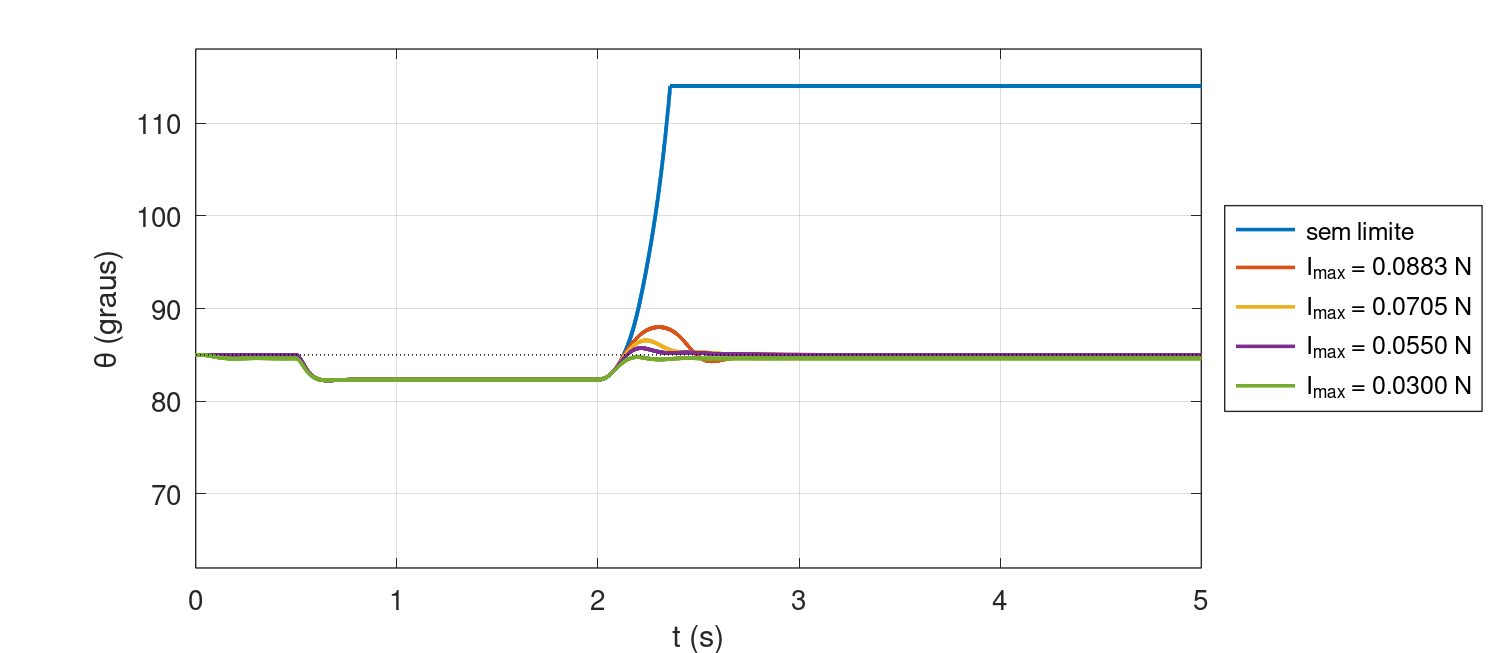
\includegraphics[width=0.80\textwidth]{fig_sim_sensibilidade.png}
\caption{Ângulo da haste com integração limitada para diferentes valores de $I_{max}$ ($I_{min}=0$).}
\label{fig:sens}
\end{figure}

\begin{table}[H]
\centering\small
\caption{Efeito do limite superior $I_{max}$ ($F_h=0{,}040$~N, $F_{max}=0{,}088$~N).}
\label{tab:sens}
\begin{tabular}{@{}lcccc@{}}
\toprule
$I_{max}$ (N) & $\theta_{max}$ ($^\circ$) & $t_r$ (s) & erro final ($^\circ$) & resultado \\
\midrule
sem limite & 114,0 & $\infty$ & 29,0 & tomba \\
0,0883 ($=F_{max}$) & 88,0 & 0,45 & 0,00 & recupera \\
0,0705 (projeto) & 86,6 & 0,31 & 0,00 & recupera \\
0,0550 & 85,7 & 0,11 & 0,00 & recupera \\
0,0300 ($<F_h$) & 84,8 & 0,12 & $-0{,}39$ & erro de regime \\
\bottomrule
\end{tabular}
\end{table}

\textbf{Conversão para o \textit{firmware}.} O \textit{firmware} trabalha com $u$ normalizado
(0 a 1 da razão cíclica útil, após a compensação da zona morta) e ângulos em graus. Admitindo empuxo
aproximadamente linear em $u$ após a compensação, com $u=1\leftrightarrow F_{max}$, os valores
acima correspondem a $K_p\approx0{,}39$/°, $K_i\approx1{,}05$/(°$\cdot$s), $K_d\approx0{,}031$/(°/s) e
$I\in[0;\,0{,}80]$. O limite atual do \textit{firmware}, $I_{max}=0{,}40$, é menor que o
$F_h/F_{max}=0{,}46$ necessário em $85^\circ$, e será corrigido após a identificação da curva de
empuxo do v2.

%%%%%%%%%%%%%%%%%%%%%%%%%%%%%%%%%%%%%%%%%%%%%%%%%%%%%%%%%%%%%%%%%%%%%%%%%%%%
\section{Modelo em Simulink}
\label{sec:simulink}

O modelo \texttt{aeropendulo.slx} implementa as equações \eqref{eq:planta}, \eqref{eq:atuador} e
\eqref{eq:il} com blocos padrão do Simulink (Figura~\ref{fig:simulink}):
\begin{itemize}
  \item \textbf{Controlador:} amostradores (\textit{Zero-Order Hold}) de $\phi$ e $\dot\phi$ com $T_s$;
    integrador discreto (\textit{Discrete-Time Integrator}, Euler regressivo) com limites de saída;
    ganhos $K_p$, $K_i$, $K_d$.
  \item \textbf{Integração limitada:} os limites de saída do integrador discreto restringem o
    \textbf{estado} do integrador, que é exatamente a técnica. Com limites $\pm\infty$, obtém-se o
    caso sem \textit{anti-windup}.
  \item \textbf{Atuador:} saturação $[F_{min},F_{max}]$ seguida da dinâmica de primeira ordem.
  \item \textbf{Haste:} dois integradores; o de posição tem os batentes do piso, e sua porta de
    saturação zera a velocidade no contato.
  \item \textbf{Perturbações:} toque (pulso de torque) e mão (mola e amortecedor ativos numa janela de
    tempo).
\end{itemize}
O solver é de passo fixo (\texttt{ode4}, 0,5~ms).

\begin{figure}[H]
\centering
\begin{tikzpicture}[node distance=6mm and 8mm, font=\footnotesize]
  \node (ref) {$\phi_r$};
  \node[sumc, right=5mm of ref] (s1) {};
  \node[blk, right=of s1, minimum width=26mm] (pid) {PID discreto\\$T_s=5$ ms, IL $[I_{min},I_{max}]$};
  \node[blk, right=of pid, minimum width=16mm] (sat) {Saturação\\$[0,F_{max}]$};
  \node[blk, right=of sat, minimum width=16mm] (mot) {$\dfrac{1}{\tau_m s+1}$};
  \node[sumc, right=7mm of mot] (s2) {};
  \node[blk, right=7mm of s2, minimum width=22mm] (rod) {Haste\\não linear};
  \node[right=6mm of rod] (out) {$\theta$};
  \node[above=5mm of s2] (d) {$\tau_d$ (toque, mão)};
  \node[blk, below=8mm of pid, minimum width=26mm] (zoh) {ZOH ($\phi$, $\dot\phi$)};
  \draw[sig] (ref) -- (s1);
  \draw[sig] (s1) -- node[above]{$e$} (pid);
  \draw[sig] (pid) -- node[above]{$u$} (sat);
  \draw[sig] (sat) -- (mot);
  \draw[sig] (mot) -- node[above]{$LF$} (s2);
  \draw[sig] (d) -- (s2);
  \draw[sig] (s2) -- (rod);
  \draw[sig] (rod) -- coordinate (tap) (out);
  \draw[sig] (tap) |- (zoh);
  \draw[sig] (zoh) -| node[pos=0.95, left]{$-$} (s1);
  \draw[sig] (zoh.north) -- node[right]{$\dot\phi$ (D)} (pid.south);
\end{tikzpicture}
\caption{Estrutura do modelo em Simulink.}
\label{fig:simulink}
\end{figure}

Os arquivos da pasta \texttt{simulacao} são:
\begin{itemize}
  \item \texttt{parametros\_aeropendulo.m}: parâmetros do modelo, do atuador e do controlador;
  \item \texttt{cria\_modelo\_aeropendulo.m}: gera o \texttt{aeropendulo.slx};
  \item \texttt{roda\_simulink.m}: roda os três casos no Simulink e compara cada resposta com a
    simulação por \textit{script};
  \item \texttt{simula\_aeropendulo.m} e \texttt{compara\_casos.m}: simulação por \textit{script},
    compatível com MATLAB e GNU Octave, sem \textit{toolboxes}.
\end{itemize}
As figuras da Seção~\ref{sec:aw} foram obtidas com a simulação por \textit{script}.

%%%%%%%%%%%%%%%%%%%%%%%%%%%%%%%%%%%%%%%%%%%%%%%%%%%%%%%%%%%%%%%%%%%%%%%%%%%%
\section{Objetivos específicos do controlador}
\label{sec:objetivos}

Com base no modelo e nas limitações medidas, os objetivos da Tabela~\ref{tab:objetivos} substituem
as metas preliminares da ideação.

\begin{table}[H]
\centering\small
\caption{Objetivos específicos do controlador (protótipo v2).}
\label{tab:objetivos}
\begin{tabularx}{\textwidth}{@{}l>{\raggedright\arraybackslash}X@{}}
\toprule
\textbf{Requisito} & \textbf{Meta} \\
\midrule
Faixa de referência & $83^\circ \le \theta_r \le 88^\circ$, definida pela serial ou pelo botão B1 \\
Erro em regime & $|e_{ss}| \le 1^\circ$ \\
Segurança & a haste \textbf{nunca} deve ultrapassar $90^\circ$ (não há empuxo para recuperá-la) \\
Sobressinal & $\le 3^\circ$ após degrau de referência, toque ou soltura pela mão \\
Acomodação & entrada definitiva na faixa de $\pm2^\circ$ em menos de 1,5~s \\
Rejeição de perturbação & recuperar toques de até 0,005~N$\cdot$m durante 0,2~s sem tombar \\
\textit{Anti-windup} & integração limitada com $F_h \le I_{max} \le F_{max}$ e $I_{min}=0$; comparar com e sem a técnica \\
Atuador & razão cíclica $\le 90\,\%$, sem inversão, \textit{driver} sem aquecimento excessivo \\
\bottomrule
\end{tabularx}
\end{table}

%%%%%%%%%%%%%%%%%%%%%%%%%%%%%%%%%%%%%%%%%%%%%%%%%%%%%%%%%%%%%%%%%%%%%%%%%%%%
\section{Próximos passos e cronograma}
\label{sec:proximos}

\textbf{Atuador.}
\begin{itemize}
  \item Substituir o L9110H por um MOSFET canal N de nível lógico (por exemplo, módulo AOD4184,
    AO3400 ou IRLZ44N), com diodo de roda livre. Como o atuador agora é unidirecional, a ponte H é
    desnecessária. O MOSFET elimina a queda de tensão e o aquecimento, e deve aumentar o empuxo.
  \item Avaliar outro motor ou outra hélice, por exemplo um motor sem núcleo 8520 com hélice de
    55--75~mm, como no projeto em PLA, se o empuxo continuar insuficiente pela
    equação~\eqref{eq:phimax}.
\end{itemize}

\textbf{Estrutura (v2).}
\begin{itemize}
  \item Haste leve em plástico ou impressa em 3D, com só a IMU e o ventilador embarcados.
  \item IMU perto do pivô: menos aceleração tangencial e vibração no acelerômetro, e menor braço de
    alavanca dos fios.
  \item Fios finos e flexíveis saindo pela altura do pivô, ao longo do eixo de giro.
  \item Nucleo, \textit{driver} e fonte fora da haste.
\end{itemize}

\textbf{Identificação, sintonia e ensaios.}
\begin{itemize}
  \item Medir $m$, $h$ e $L$, e obter $J$ pelo período de oscilação da haste pendurada como pêndulo
    simples.
  \item Medir de novo a curva de empuxo e a constante $\tau_m$ (degrau de PWM).
  \item Atualizar o modelo e o Simulink, e ajustar os ganhos na ordem $K_p\rightarrow K_d\rightarrow K_i$.
  \item Comparar experimentalmente o controle com e sem integração limitada, na partida pelo botão
    e no toque.
\end{itemize}

\begin{table}[H]
\centering\small
\caption{Cronograma até a entrega final (datas do plano de ensino).}
\label{tab:cronograma}
\begin{tabular}{@{}ll@{}}
\toprule
\textbf{Período} & \textbf{Atividade} \\
\midrule
11/11 & TP2: apresentação do protótipo v1 e este relatório parcial \\
12/11 -- 18/11 & compra e montagem do MOSFET; nova curva de empuxo; escolha do motor \\
16/11 -- 22/11 & impressão e montagem da estrutura v2 (fiação externa) \\
23/11 -- 29/11 & identificação ($m$, $h$, $L$, $J$, $\tau_m$, curva de empuxo); atualização do modelo \\
30/11 -- 06/12 & sintonia do PID; ensaios com e sem \textit{anti-windup}; métricas no aplicativo \\
07/12 -- 11/12 & TP3: relatório final (prazo 11/12) \\
14/12 ou 16/12 & TP4: apresentação, teste de funcionamento e arguição \\
\bottomrule
\end{tabular}
\end{table}

%%%%%%%%%%%%%%%%%%%%%%%%%%%%%%%%%%%%%%%%%%%%%%%%%%%%%%%%%%%%%%%%%%%%%%%%%%%%
\section{Conclusões parciais}

\begin{itemize}
  \item \textbf{O que foi validado.} O protótipo v1 validou o sensor, o \textit{firmware}, o
    acionamento e as ferramentas de ensaio. O sistema está pronto para receber a nova mecânica.
  \item \textbf{O que impediu o equilíbrio.} Os ensaios mostraram que o equilíbrio depende de uma
    relação favorável entre empuxo e torque da gravidade, que o v1 não atendia.
  \item \textbf{Mudanças de projeto.} Os ensaios levaram a dois redesenhos: atuador unidirecional,
    operando abaixo da vertical, e estrutura leve com a eletrônica fora da haste.
  \item \textbf{\textit{Anti-windup}.} Com o atuador unidirecional, ultrapassar a vertical é fatal, e
    a partida pelo botão satura o atuador. Nessas condições, a integração limitada passa a ser
    \textbf{necessária para a operação}, e não só uma melhoria de desempenho: na simulação, ela evita
    a queda após a haste ser solta, com sobressinal de $1{,}6^\circ$ e recuperação em 0,31~s.
\end{itemize}

\begin{thebibliography}{9}\small
\bibitem{ogata} K. Ogata, \textit{Engenharia de Controle Moderno}, 5.\textsuperscript{a} ed. São Paulo: Pearson, 2010.
\bibitem{franklin} G. F. Franklin, J. D. Powell, A. Emami-Naeini, \textit{Sistemas de Controle para Engenharia}, 6.\textsuperscript{a} ed. Porto Alegre: Bookman, 2013.
\bibitem{astrom} K. J. Åström, T. Hägglund, \textit{Advanced PID Control}. ISA, 2006.
\bibitem{visioli} A. Visioli, \textit{Practical PID Control}. London: Springer, 2006.
\bibitem{equipe} D. B. N. Buente, J. P. P. A. Santos, ``\textit{Anti-windup} por integração limitada aplicado ao controle de ângulo de um aeropêndulo'', trabalho AS, ENGC54, UFBA, 2026.
\bibitem{st} STMicroelectronics, \textit{UM1724 -- STM32 Nucleo-64 boards user manual}.
\bibitem{mpu} InvenSense, \textit{MPU-9250 Product Specification}, rev. 1.1, 2016.
\end{thebibliography}

\end{document}
